\chapter{Background}
%-Available spike analysis frameworks \\
%-fieldtrip \\\
%-elephant \\
%-Why they are not sufficient \\
%-problem with the relays? maybe windows updates 

%-openMNGlab as a solution \\
%-acquisition frameworks we need to handle \\
%-Current status of openMNGlab, including Neo \\
%-go into detail on different data acquisition softwares \\
%-Dapsys, OpenEphys, Spike2 \\
%-why does dapsys not work in the future \\

\section{Analysis tools}
When it comes to analysis software for microneurography data,  there are multiple available that each have their own use-cases.

\subsection{FieldTrip}
Fieldtrip (fieldtriptoolboX.org) is a MATLAB toolbox developed at the Radboud University,  Nijmegen,  the Netherlands and offers a wide variety of analysis functions.  It can analyse MEG, EEG, and iEEG and is an open-source software that has been in development since 2003. Its main strengths lie in the analysis of non-invasive and invasive electrophysiological data. It provides over 100 high-level and 800 low-level functions that can be used both by experimental users as well as developers. It does not feature a graphical user interface, but instead focuses on providing direct access to the high and low-level analysis functions that can be used in the command line or in scripts.  This increases flexibility and is done because FieldTrip is not meant to be an application but a set of tools that can be mixed and matched for different requirements.
With this approach the user needs to be somewhat familiar with MATLAB before starting their analysis, but after a potential initial time invest the flexibility of this approach yields great advantages.
The analysis functions are meant to be combined and used as a sort of analysis protocol, where the output of functions is used to compute the next results. 
An example pipeline is lined out in the paper (put citation here). The first step after loading the data set of interest is to choose a data segment that is to be analysed by setting the boundaries of said segment. In order to free the data from noise and artifacts that could compromise the analysis. FieldTrip provides the corresponding functions for automatic removal of artifacts. As a next step the user can run a preprocessing function that loads the specified data into the MATLAB workspace and readies it for further analysis. Then the user can choose which specific analysis they want to perform. There is also the possibility of source reconstruction to get a visual representation of the source of the data.\\
An important feature of FieldTrip is the ability to save and reuse intermediate results. After each step in the analysis there is the possibility to save the current results for later use before further altering the data. This can be useful in many situations where the user wants to retrace certain steps in the analysis.\\
For visualization of results users can make use of standard MATLAB functionalities to plot the numeric results of FieldTrip analyses.\\
As an open-source software FieldTrip is also meant to be contributed to by developers who see opportunities for improvement. As opposed to other GUI-using software FieldTrips focus on having the direct access to functions lends itself to development and icontributions from various different experts, which only enhance the product.

This software package is very useful and widely used in the field, however it does not lend itself to our specific needs.
The main problem with this software is its programming language. It is a MATLAB toolbox, however it would be preferred to use a software package in python or another programming language that slots better in the already existing structure that is used at the chair for medical informatics.  

\begin{comment}
\subsection{Elephant}
Elephant (https://elephant.readthedocs.io/en/latest/index.html) is a python module which offers some high-level analysis functions for spike trains specifically.  The main problem with this software is the lack of basic functionalities.  It relies more on highly specified analysis tools that are not necessarily viable in our use-case.  For the use in this thesis I want to start with the basic signal from the spikes, try out different quantifiers and look at the data from a fresh perspective. 
\end{comment}
\subsection{openMNGlab}
The previously presented analysis tools could not be used for this thesis for different reasons.
There are multiple data acquisition systems that are used at the chair of IMI that each produce different file formats.. The three main systems that need to be handled are Spike2, Dapsys and OpenEphys and are described in more detail in the next section. \\ 
We need a tool that that has the capability to load files from these different data acqusition softwares, put them in a compatible format and analyse them further.  FieldTrip does not offer these kinds of capabilities as well as it being a MATLAB package, which would not be ideal for fitting into the rest of the analysis systems at IMI. Elephant is also lacking the importing tools that would be required for the software solution.  \\
For this reason the Institute of medical informatics has started to develop their own software framework in python called openMNGlab.  This framework aims to provide a solution for those issues with the different file types and combine them into a single usable format.  In addition it provides analysis capabilities for microneurography data. \\
For the import of the different file types from the data acqusition packages and the internal structure of the data openMNGlab makes use of an already developed python module called Neo(neuralensemble.org/neo). This is a package that already deals with neurophysiological data in various different file formats. It is aimed towards combining these different sources while not providing any analysis capabilities of its own to reduce dependencies (cite website here). It also comes with templates to build importers for different new file formats should those be required and thus makes it easier to include more file formats at a later date.\\
OpenMNGlab has started as a project of the Institute of medical informatics and was initially developed by Fabian Schlebusch who developed openMNglab 1.0 and setup the basic structure and developed the importers necessary for the file formats that we require. \\
However, the 1.0 version of the framework is not enough in terms of analysis and also importing capabilities and needs to be improved. 

At IMI there are people who work on varying aspects of MNG data analysis such as analyzing the response latency to electrical stimulation or analyzing the nerve activity in response to certain chemicals. I am focusing on analyzing spike trains occuring in mechanically and electrically stimulated nerve fibers.\\
With my bachelor thesis I aim to provide some more analysis functionalities for spike trains as well as give some ideas on the software engineering of the software framework in the future.\\
In the end FieldTrip and Elephant offer good solution for slightly different use-cases, but were not a perfect fit for the analysis of microneurography data at the Institute of medical informatics. They are, however, a good inspiration for what should be included in such a software framework. In the case of Elephant, since it is also a python module and also makes use of the Neo structure, it could make for a good addition of more high-level analysis functionalities in the future.


\begin{comment}
Neo:\\
brings a data structure\\
importers or at least templates for importers

As mentioned before, Neo is the basis of openMNGlab when it comes to the structure of the data. It provides a common ground for electrophysiological data from different sources. It 
Because it is meant to be used in conjunction with many different file formats, it already comes with importing functionalities for a couple of formats. In addition to the already available importers, Neo provides the tools to write new importers for file formats which are not already supported. These templates are the basis of the importers in openMNGlab.
\end{comment}



\section{Data acquisition software} 
A data acquisition system is a combination of software and hardware components that work together in order to control inputs towards and record data from different subjects.
There are many different data acquisition systems for electrophysiological data. There are three systems that we are working with and that should be compatible with our chosen software analysis framework. These systems are Spike2, Dapsys and OpenEphys.

\subsection{Spike2}
%“Spike2 is a multi-channel continuous data acquisition and analysis package”( https://ced.co.uk/products/spkovin) produced by Cambridge electronic design limited. \\
%-Used for the experiments I am analysing by Roberto \\
%-records data in multiple channels \\
%-channel for raw signal \\
%-channel for mechanical force \\
%-channel for event markers \\
%-channel for temperature (not used by me) \\
%-channel for comments (used for marking when chemicals are applied) \\
%-spikes can be separated into own channels (done by experimenters) \\
%-software offers a graphical representation of the data \\
%-channels are separated \\
%-was used for confirmation of what the data should output in terms of basic quantifiers \\
%-can export csv files from the data \\
%-has direct importer in openMNGlab \\

Spike2 is a data acquisition and analysis software produced by Cambridge electronic design limited. It is a flexible tool that can be used in a variety of different ways.

\begin{figure}
	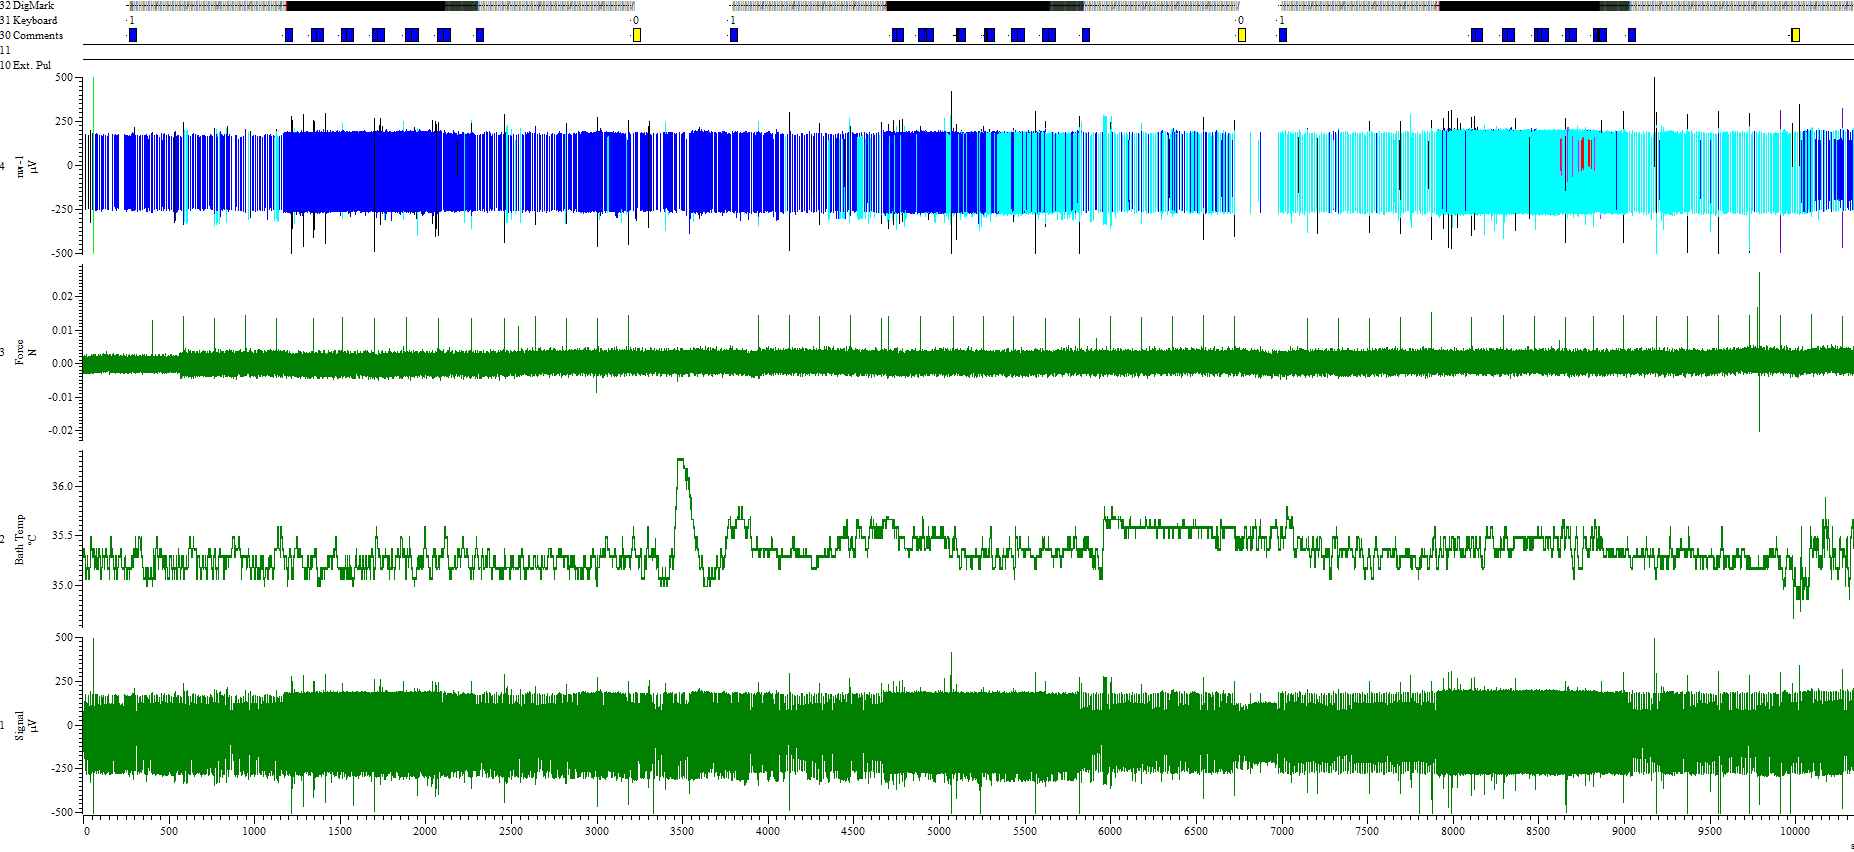
\includegraphics[width = \textwidth]{src/pic/Spike2_screenshot}
	\caption{Typical mechanically and electrically stimulated recording in Spike2}
	\label{fig:spike2}
\end{figure}

The software can record multiple channels simultaneously. An example screenshot from a recording can be seen in Figure~\ref{fig:spike2}. This depicts a typical recording used for analysis in this bachelor thesis. The recording contains data from nerve fibers of rat cranial dura mater. The nerve fibers were stimulated using a mechanoelectrostimulator applying electaical and mechanical stimulation. 

\begin{figure}
	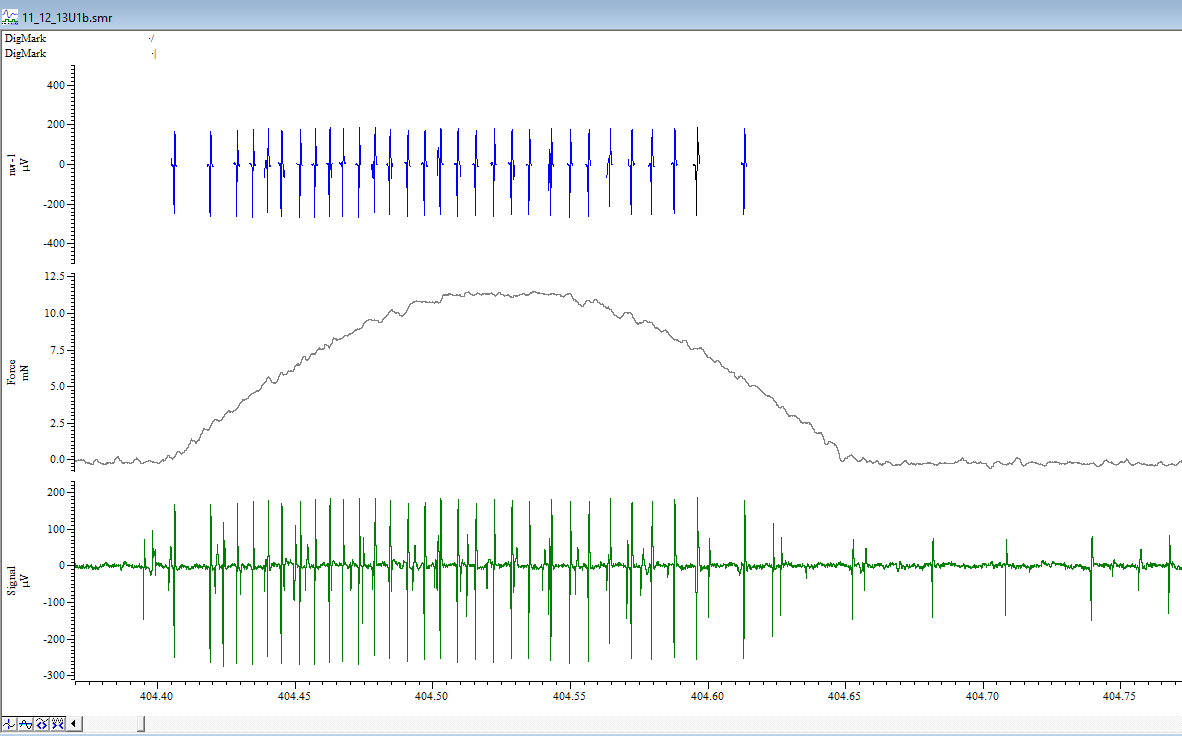
\includegraphics[width = \textwidth]{src/pic/Spike2_spike_train}
	\caption{A single spike train in spike2}
	\label{fig:spike_train}
\end{figure}

First of all it contains a channel for the recorded raw signal at the bottom. The next channel contains the temperature during the recording. In this example it fluctuates between 35°C and 36.5°C. In channel 3 we can observe the mechanical force that was applied to the nerve fibers. In Figure~\ref{fig:spike2} there are spikes in mechanical force whenever a mechanical stimulation occurs to evoke a spike train. For this experiment we want to collect the data of single nerve fibers. It is diffucult, to record just a single nerve fiber in vitro, however. This is why in this experiment spike templates are applied to the raw signal to filter out specific fibers. These filtered fibers are then displayed in so called wavemark channels. In this example channel 4 is such a channel, where only specific action potentials are filtered. The filtering process is done by the experimenters and is based on certain features of the action potential shape.\\
The topmost channel in Figure~\ref{fig:spike2} contains markers for the electrical and mechanical stimuli. Additionally there is a channel containing comments regarding the experiment. Comments can represent the experimental protocol and are filled in by the experimenters. In this example there are comments denoting a change electrical stimulation frequency. In other experiments for example, these could also denote the application of certain chemicals towards the recorded subject.

A more detailed view of a single spike train can be seen in Figure~\ref{fig:spike_train}. Here the difference in electrical and mechanical event markers in the topmost channel can be seen. Mechanical markers are represented by a slash, while electrical markers are represented by a vertical line. Another thing that can be seen here is the channel containing only the spikes. This channel is ideal for the extraction of the spikes for later analysis as there is no noise in the channel anymore and the spikes can also be interpreted as simple events with a timestamp.

\subsection{Dapsys}
%“DAPSYS is a combined hardware and software system designed for real-time acquisition and display of data and synchronous %control of stimulators.” (http://www.dapsys.net/) \\
%-Used by Barbara for her experiments \\
%-used for mng-experiments with human patients \\
%-also has a graphical representation of the data \\
%-has importer in openMNGlab \\
%-needs to export specific templates as csv for the importer to work \\
%-Dapsys has problem in the future \\
%-it gets harder to set up experimental protocols \\
%-maybe it has something to do with newer windows updates \\
%-that means this will probably not be used much in the future \\
%http://www.dapsys.net/rd_article/rd_article.html

The second data acquisiton package that openMNGlab needs to support is called Dapsys. It is a hardware and software system that can record and analyse electrophysiological data from animal or human sources and has been mainly used for studying the peripheral nervous system (cite website here). It has been in development for over 30 years since its earliest version and thus has a great history of usage in the field. The idea behind the conception was to build a system that could control stimulators and simultaneously acquire the data in real-time and display the data (cite the article).\\
Dapsys offers the capabilities of path tracking and comes with the benefit of much data being available from experiments conducted with the Dapsys software. It is used especially for electrophysiological recordings with human patients. As is the case for Spike2 it also comes with a visual representation of the data which can be seen in Figure~\ref(dapsys). This graphical interface works real time while recording the data.\\
\begin{figure}
	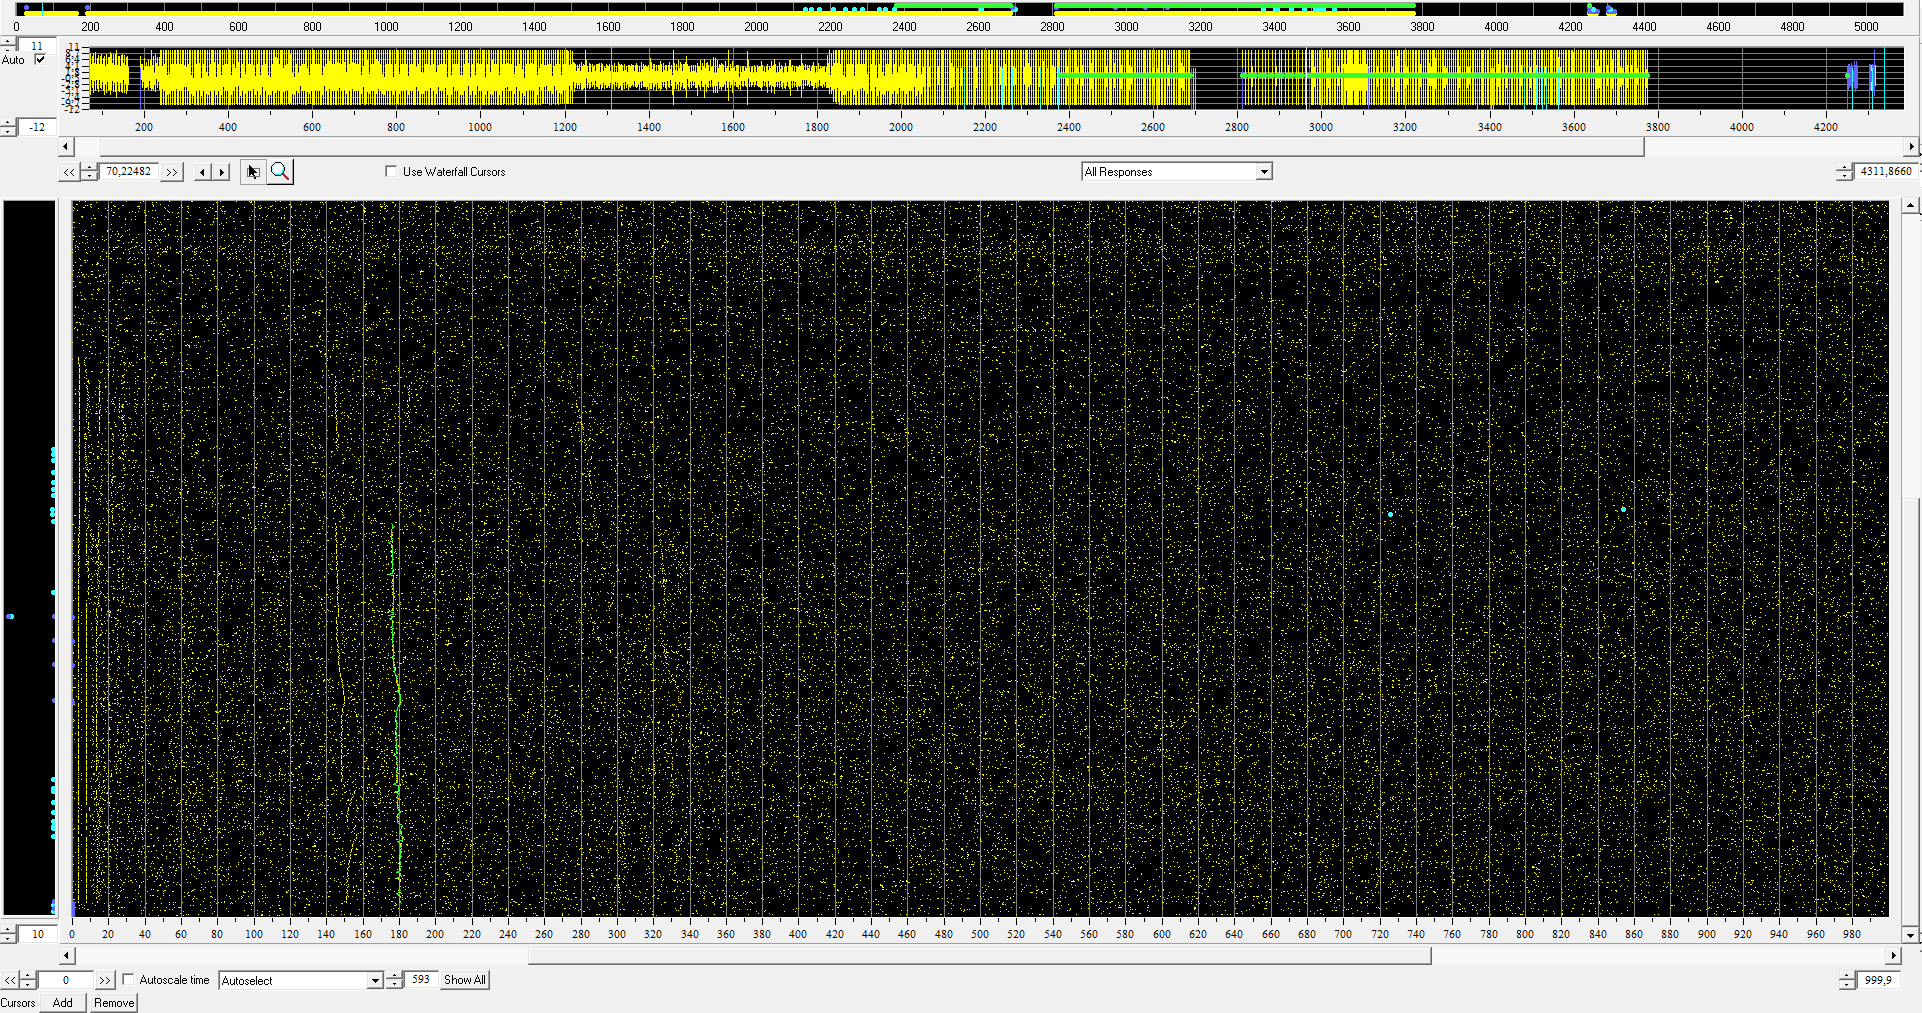
\includegraphics[width = \textwidth]{src/pic/Dapsys_sc}
	\caption{Screenshot of a recording in Dapsys}
	\label{fig:dapsys}
\end{figure}
The version of Dapsys used in the experiments from Barbara Namer is specialized for microneurography and was configured in cooperation with Brian Turnquist.\\
OpenMNGlab already features an importer for Dapsys recordings, which makes many experiments conducted with this system readily available for analysis.
The difference to Spike2 however, is that the importer does need an extra step from the user, since it does not import the raw Dapsys files. We need to export the raw data and templates for the tracks we want to analyse as csv files from the Dapsys software, before we can import them into openMNGlab. This process is especially combersome when dealing with a larger number of recordings. In the future the importer functionality of openMNGlab should be improved, so that it works on the raw Dapsys files in order to make the analysis workflow easier.\\


\subsection{OpenEphys}
%OpenEphys \\
%-open-source electrophysiology \\
%-based in Cambridge, Massachusetts \\
%-Used in experiments in Bristol cooperation \\
%OpenEphys is an open-source electrophysiology data acqusition software from a nonprofit based in Cambridge, Massachusetts. Its aim is that in the future neuroscientists can choose the right tool for their job and that there are many tools available. This is best accomplished by providing open-source solutions.\\
%They provide a platform where researchers can individually choose their own experimental setup from a number of different open-souce and other components.
%OpenEphys is used by one of the collaborators of IMI in Bristol.

The last data acquisition system I want to focus on is called OpenEphys. It is an open-source electrophysiology data acquisition system originally developed by a nonprofit based in Cambridge, Massachusetts. It sets a big focus on modularity and flexibility so that it can fit many different needs from a variety of users.\\

The idea behind OpenEphys came after an increased popularity of closed-loop experiments in neuroscience, in which the results of the recorded system has an influence on the system itself. With proprietary systems it is somewhat difficult to share the details of such experiments and to replicate them. The introduction of OpenEphys, an open-source system is supposed to make it easier to develop and share analysis and details of such closed-loop experiments.\\
OpenEphys makes use of inexpensive open-source hardware such as Intan chips to make it easier for small labs to get started with analysing electrophysiological data. The heart of the software part of the system is a plugin-based graphical user interface (GUI). Here the user can add different modules to the processing pipeline such as modules for communicating with the hardware or modules for analysing the data.\\
Different labs often have widely varying sets of requirements towards data analysis and therefore data acquisition systems. At the start of a project they are confronted with the question of whether to use a proprietary system or develop their own systems, which will result in much more effort before the real work can begin. Proprietary systems also often come with very limited customization possibilities, which makes it harder to get the system that fits the users needs exactly. This is where OpenEphys comes in with its plugin-based software. It is designed so that everyone can mix and match the processing modules and end up with the exact analysis pipeline that they require. In addition to a wide array of already available processing modules, it is possible to develop your own modules that fit seamlessly into the structure of the system. OpenEphys is completely developed in C++ and based on a library for audio applications. This makes it easy to develop new modules by making use of the class inheritance capabilities of C++.\\
OpenEphys comes with many advantages such as low cost, transparency and flexibility due to the modularity, but there are also drawbacks to using the system. The start is also a little harder than in proprietary systems, where there is often a straight forward way of getting started with your first experiments. The modular nature of the system might also effect the performance of the analysis, which is why commercial systems might be a better choice, if they fit the analysis needs.\\

In this thesis we are considering OpenEphys because it is used by a collaborating research team in Bristol, which also wants to make use of openMNGlab.



 
\cleardoublepage
